\section{Hankel alternative view of Koopman with control} 
\label{sec:havok}
    
    \paragraph
    \gls{HAVOK} is a data-driven, regression technique that provides a different approximation
    of the Koopman operator than \gls{DMD} \cite{Brunton2017a, Champion2019}. 
    The Koopman operator is a method of representing finite-dimensional non-linear dynamics
    in terms of an infinite-dimensional linear operator \cite{Brunton2017a}.
    However, an infinite-dimensional linear operator is not very useful for practical implementation.
    \gls{DMD} provides a limited approximation of the Koopman operator, because it is based on linear measurements only.
    \gls{HAVOK} was developed to improve the Koopman approximation of \gls{DMD} by using intrinsic measurement coordinates based on the time-history of the system \cite{Brunton2017a}.
    
    \paragraph
    The original formulation of \gls{HAVOK} is only defined for uncontrolled dynamical systems \cite{Brunton2017a}.
    In this work, we have adapted the standard \gls{HAVOK} algorithm to account for the effect of control.
    This implementation well be referred to as \gls{HAVOKc}.
    This algorithm results in a discrete, linear model that approximates the behaviour of a controlled dynamical system.
    In this section, a brief overview is provided of this implementation of \gls{HAVOKc}.
    
    \paragraph
    A defining characteristic of \gls{HAVOK} is that it uses multiple delay-coordinates (i.e. $\bm{x}_{k-1}, \bm{x}_{k-2}$, etc.) 
    in the system identification process.
    To fit this into the standard state-space format, an extended state vector is defined as:
    \begin{equation}
         \bm{a}_{k} = \begin{bmatrix} \bm{x}_{k-(q-1)} & \cdots & & \bm{x}_{k-1} & & \bm{x}_{k} \end{bmatrix}^T ,
    \end{equation}
    where $\bm{a}_k \in \R^{(n_y)(q)}$, and the subscript of $\bm{a}$ denotes the highest subscript of ${\bm{x}}$ in the vector.
    
    \paragraph
    The resulting discrete state-space model is therefore in the form,
    \begin{equation} \label{eq:havok_state_space}
        \bm{a}_{k+1} = \bm{A}_H \bm{a}_k + \bm{B}_H \bm{u}_k ,
    \end{equation}
    where \( \bm{A}_H \in \R^{(q \cdot n_x) \times (q \cdot n_x)} \) is the system matrix, 
    and \( \bm{B}_H \in \R^{(q \cdot n_x) \times n_u} \) is the input matrix. 
    % 
    \paragraph
    The original \gls{HAVOK} algorithm, developed by \citet{Brunton2017a}, constructs a Hankel matrix from output variables only. 
    In this work, the standard \gls{HAVOK} algorithm has been adapted to incorporate the effect of control.
    An extended Hankel matrix, $\bm{\Pi}$, is created by appending a matrix of inputs to a Hankel matrix of measurements:
    \begin{equation} \label{eq:pi_hankel}
        \bm{\Pi} = \phantom{.} \left [
            \begin{array}{*{5}{@{}M{\mycolwd}@{}}}
                    \bm{a}_{q} & \bm{a}_{q+1} & \bm{a}_{q+2} & \cdots & \bm{a}_{w+q-1} \\
                    \bm{u}_{q} & \bm{u}_{q+1} & \bm{u}_{q+2} & \cdots & \bm{u}_{w+q-1}
            \end{array}
        \right ] ,
    \end{equation}
    where $w$ is the number of columns in $\bm{\Pi}$.
    A truncated \gls{SVD} of this Hankel matrix results in following approximation:
    \begin{equation} \label{eq:havok_svd_tilde}
        \bm{\Pi} \approx \Tilde{\bm{U}} \Tilde{\bm{\Sigma}} \Tilde{\bm{V}}^T ,
    \end{equation}
    where $\Tilde{\phantom{a}}$ represents rank-$p$ truncation.
    It is important to note that the model extracted by \gls{HAVOKc} depends on the choice of hyperparameters ($p$ and $q$),
    and the number of training samples ($N_{train} = w + q -1$).
    
    \paragraph
    The columns of $\Tilde{\bm{V}}$ are the most significant principal components of the system dynamics \cite{Kamb2020}.
    This matrix, $\Tilde{\bm{V}}$, can be considered to contain a time-series of the pseudo-state, $\bm{v}$, such that
    \(
        \Tilde{\bm{V}}^T = \begin{bmatrix} 
            \bm{v}_q & \bm{v}_{q+1} & \cdots & \bm{v}_w 
        \end{bmatrix} ,
    \)
    characterises the evolution of the actual dynamics in an eigen-time-delay coordinate system \cite{Brunton2017a}.
    % 
    Consider the following discrete, state-space formulation:
    \begin{equation} \label{eq:v_ss}
        \bm{v}_{k+1} = \bm{\Lambda} \bm{v}_k .
    \end{equation}
    \gls{HAVOKc} determines the best fit linear operator $\bm{\Lambda}$ that maps the pseudo-state $\bm{v}_k$ to $\bm{v}_{k+1}$.
    In order to setup an over-determined equality for Equation~\ref{eq:v_ss}, $\Tilde{\bm{V}}^T$ is divided into two matrices:
    \begin{align} \label{eq:v1v2}
        \bm{V}_1 &= \left [
            \begin{array}{*{5}{@{}M{\mycolwd}@{}}} 
                \bm{v}_{q \phantom{-1}}     & \bm{v}_{q+1} & ... & \bm{v}_{w-1} \\
            \end{array} 
        \right ] , \nonumber \\ 
        \bm{V}_2 &= \left [
            \begin{array}{*{5}{@{}M{\mycolwd}@{}}} 
                \bm{v}_{q+1}     & \bm{v}_{q+2} & ... & \bm{v}_{w \phantom{-1}} \\
            \end{array} 
        \right ] ,
    \end{align} 
    where $\bm{V}_2$ is $\bm{V}_1$ advanced a single step forward in time.
    The matrices from Equation~\ref{eq:v1v2} are now combined with Equation~\ref{eq:v_ss} and the best fit $\bm{\Lambda}$ is determined with the Moore-Penrose pseudoinverse:
    \begin{equation} \label{eq:v_dmd}
        \bm{V}_2 = \bm{\Lambda} \bm{V}_1 \phantom{---} \Rightarrow \phantom{---} \bm{\Lambda} \approx \bm{V}_1 \bm{V}_1^{\dagger}
    \end{equation}
    % 
    It can be shown from Equation~\ref{eq:havok_svd_tilde} that Equation~\ref{eq:v_ss} is transformed from the eigen-time-delay coordinate system to the original coordinate system as the following:
    \begin{equation} \label{eq:v_ss_a} 
        \begin{bmatrix}
            \bm{a}_{k+1}  \\  \bm{u}_{k+1} 
        \end{bmatrix}
    \phantom{.} = \phantom{.} (\Tilde{\bm{U}} \Tilde{\bm{\Sigma}}) \bm{\Lambda} (\Tilde{\bm{U}}  \Tilde{\bm{\Sigma}})^{\dagger} \phantom{.}
        \begin{bmatrix}
            \bm{a}_{k}  \\  \bm{u}_{k} 
        \end{bmatrix} .
    \end{equation}    
    % 
    % This form is used to extract $\bm{A}_H$ and $\bm{B}_H$ from the matrix,
    % \( 
    %     (\Tilde{\bm{U}} \Tilde{\bm{\Sigma}}) \bm{\Lambda} (\Tilde{\bm{U}}  \Tilde{\bm{\Sigma}})^{\dagger}
    % \), in the following way:
    % \begin{equation} \label{matrix_decomp}
    %     \begin{bmatrix}
    %         \bm{a}_{k+1}  \\  \bm{u}_{k+1} 
    %     \end{bmatrix}
    %     \phantom{.} = \phantom{.} 
    %     \begin{bmatrix}
    %         \bm{A}_H \phantom{.....} \bm{B}_H \\
    %         \textit{(discarded)}
    %     \end{bmatrix}
    %     \phantom{.}
    %     \begin{bmatrix}
    %         \bm{a}_{k}  \\  \bm{u}_{k} 
    %     \end{bmatrix}.
    % \end{equation}    
    
    \paragraph
    $\bm{A}_H$ and $\bm{B}_H$ can now be extracted from the matrix,
    \( 
        (\Tilde{\bm{U}} \Tilde{\bm{\Sigma}}) \bm{\Lambda} (\Tilde{\bm{U}}  \Tilde{\bm{\Sigma}})^{\dagger}
    \).
    This extraction is illustrated in Figure~\ref{fig:havok_decomposition}, 
    where different blocks represent different groups of matrix entries.
    \begin{figure}[htb]
        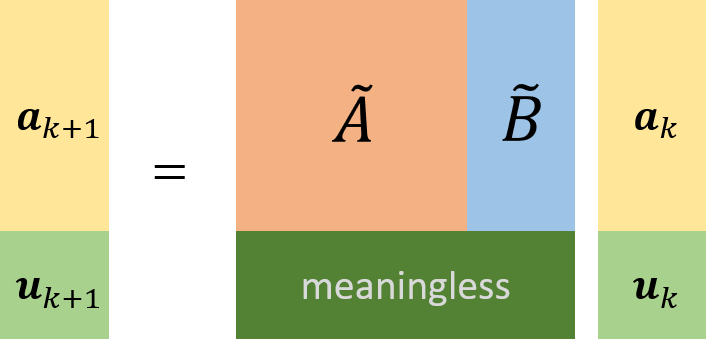
\includegraphics[scale = 0.55]{havok_decomposition.png}
        \centering
        \caption{Illustration of the extraction of $\bm{A}_H$ and $\bm{B}_H$ from Equation~\ref{eq:v_ss_a}}
        \label{fig:havok_decomposition}
    \end{figure}
    
    \paragraph
    Note that the matrix entries in Figure~\ref{fig:havok_decomposition} that map $\bm{u}_k$ to $\bm{u}_{k+1}$ 
    are meaningless for state predictions and are discarded.
    Also note that the state vector, $\bm{a}_k$, includes delay-coordinates, therefore some matrix entries are independent of the dynamics.
    This is illustrated in Figure~\ref{fig:havok_force_entries} for an example model with $q = 4$.
    For example, the mapping of $\bm{x}_k$ in the state vector to $\bm{x}_k$ in the predicted state vector
    corresponds to a entry of 1 in the $\bm{A}_H$ matrix.
    This is fixed by the model format and is not a function of the system dynamics.
    Due to the least-squares fitting and the coordinate transformation of the algorithm, 
    \gls{HAVOKc} does not produce these exact values in $\bm{A}_H$ and $\bm{B}_H$. 
    By forcing each of these matrix entries to 1 or 0, the state-prediction performance of the model is improved.
    Finally, the improved $\bm{A}_H$ and $\bm{B}_H$ are inserted into Equation~\ref{eq:havok_state_space} to render the \gls{HAVOKc} model.
        
    \begin{figure}[htb]
        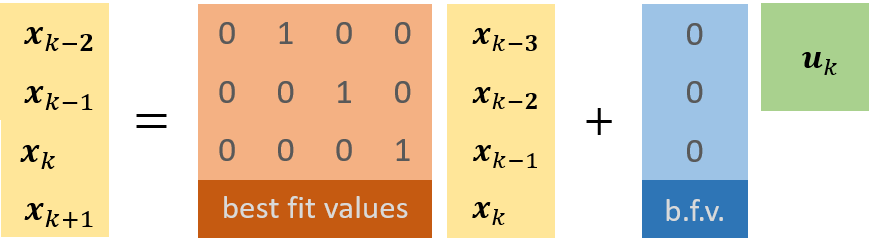
\includegraphics[scale = 0.75]{havok_force_entries.png}
        \centering
        \caption{Illustration of forcing the known values in \gls{HAVOKc} matrices}
        \label{fig:havok_force_entries}
    \end{figure}

    \paragraph
    For a high-level comparison of the data-driven methods, recall from Section~\ref{sec:dmdc} that \gls{DMDc} applies least-squares regression directly to the collected state and input data matrices.
    \gls{HAVOKc} first applies an \gls{SVD} to the state and input data, and truncates the insignificant modes.
    Least-squares regression is then applied to the pseudo-state data from the truncated \gls{SVD} to determine a state-space model.
    This model is then transformed back into the original coordinate frame.




